\section{Geometry}
    
\subsection{Pythagorean Triples}

For all natural $a, b, c$ satisfying $a^2 + b^2 = c^2$ there exist $m, n \in \mathbb{N}$ and $m > n$ such that (reverse is also true):
$$a = m^2 - n^2 \qquad b = 2mn \qquad c = m^2 + n^2$$

\subsection{Heron's Formula}

The area of a triangle can be written as $A = \sqrt{s\,(s-a)\,(s-b)\,(s-c)}$, where $a, b, c$ are the lengths of its sides and $s = \frac{a+b+c}{2}$.

This can be generalized to compute the area $A$ of a quadrilateral with sides $a, b, c, d$, with $s = \frac{a+b+c+d}{2}$ and $\alpha, \gamma$ any two opposite angles:

$$ A = \sqrt{(s-a)(s-b)(s-c)(s-d) - abcd\left( \cos ^2 \left( \frac{\alpha+\gamma}{2} \right) \right)} $$

\subsection{Pick's Theorem}

The area of a simple polygon whose vertices have integer coordinates is:

\[
A = I + \frac{B}{2} - 1
\]

where $I$ is the number of interior integer points, and $B$ is the number of integer points in the border of the polygon.

\subsection{Colinear Points}

Three points are colinear on $\mathbb{R}^2$ iff:

$$ \begin{vmatrix}
x_A & y_A & 1 \\
x_B & y_B & 1 \\
x_C & y_C & 1 \\
\end{vmatrix}  = 0 $$

The absolute value of this determinant is twice the area of the triangle $ABC$.

\subsection{Coplanar Points}

Four points are coplanar in $\mathbb{R}^3$ iff:

$$ \begin{vmatrix}
x_A & y_A & z_A & 1 \\
x_B & y_B & z_B & 1 \\
x_C & y_C & z_C & 1 \\
x_D & y_D & z_D & 1 \\
\end{vmatrix}  = 0 $$

\subsection{Trigonometry}

\subsubsection{Angle Sum}

$$ \sin(a \pm b) = \sin a \cos b \pm \cos \ \sin b $$
$$ \cos(a \pm b) = \cos a \cos b \mp \sin a \sin b $$
$$ \tan (a \pm b) = \frac{\tan a \pm \tan b}{1 \mp \tan a \tan b}$$

\subsubsection{Sum-to-Product Transformation}

$$ \sin a \pm \sin b = 2 \sin\frac{a \pm b}{2} \cos\frac{a \mp b}{2} $$
$$ \cos a + \cos b = 2 \cos\frac{a+b}{2} \cos\frac{a-b}{2} $$
$$ \cos a - \cos b = -2 \sin\frac{a+b}{2} \sin\frac{a-b}{2} $$
$$ \tan a \pm \tan b = \frac{\sin(a \pm b)}{\cos a \cos b} $$

\subsection{Centroid of a polygon}

The coordites of the centroid of a non-self-intersecting closed polygon is:

$$ \frac{1}{3A} \left(\sum_{i = 0}^{n-1}(x_i+x_{i+1})(x_iy_{i+1} - x_{i+1}y_i) , \sum_{i = 0}^{n-1}(y_i+y_{i+1})(x_iy_{i+1} - x_{i+1}y_i) \right), $$

where $A$ is twice the signed area of the polygon.

\subsection{Two Ears Theorem}

Every simple polygon with more than 3 vertices has at least two non-overlapping ears (a ear is a vertex whose diagonal induced by its neighbors which lies strictly inside the polygon). Equivalently, every simple polygon can be triangulated. Example of a simple polygon with exactly two ears:

\begin{center}
    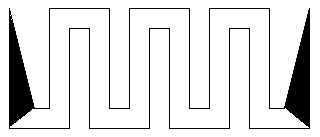
\includegraphics[width=5cm]{img/two_ears.png}
    \end{center}